% Was in the wrong place but might like to potentially add back later

In the early days of the Processing project, community interactions predominantly took place on forums. These forums, essential for user engagement, evolved in tandem with the versions of the Processing software. Each significant update of Processing was paralleled by a new iteration of the forum, starting from the Processing alpha forum and evolving through beta, 1.0, 2.0 and 3.0 versions, up to the current Processing forum. This progression reflects the software’s development and marks distinct phases in the community's journey. The chronological details of these forum versions, including the years of operation and corresponding URLs, are outlined in Table \ref{table:forums}. \parencite{ProcessingForum}

\todo[inline]{Better integrate this part}
Ben Fry is the most active forum contributor, but the activity distribution is more balanced than in Git commits, possibly due to the diverse topics covered, including technical queries and bugs. A total of 1,039 individuals contributed to the forum discussions as shown in Figure~\ref{fig:processing-alpha-dot}.
Linus's Law—"Given enough eyeballs, all bugs are shallow" \parencite[29]{raymondCathedralBazaar1999}—is somewhat evidenced by increased forum activity during release periods, suggesting community involvement in bug identification, as demonstrated in Figure~\ref{figure:forum-git-activity}.

\begin{figure}[!htbp] 
    \centering 
    %\includesvg[pretex=\sffamily\fontsize{5.58pt}{8pt}\selectfont, width=1\textwidth, keepaspectratio]{images/figure-forum-git-activity.png}
    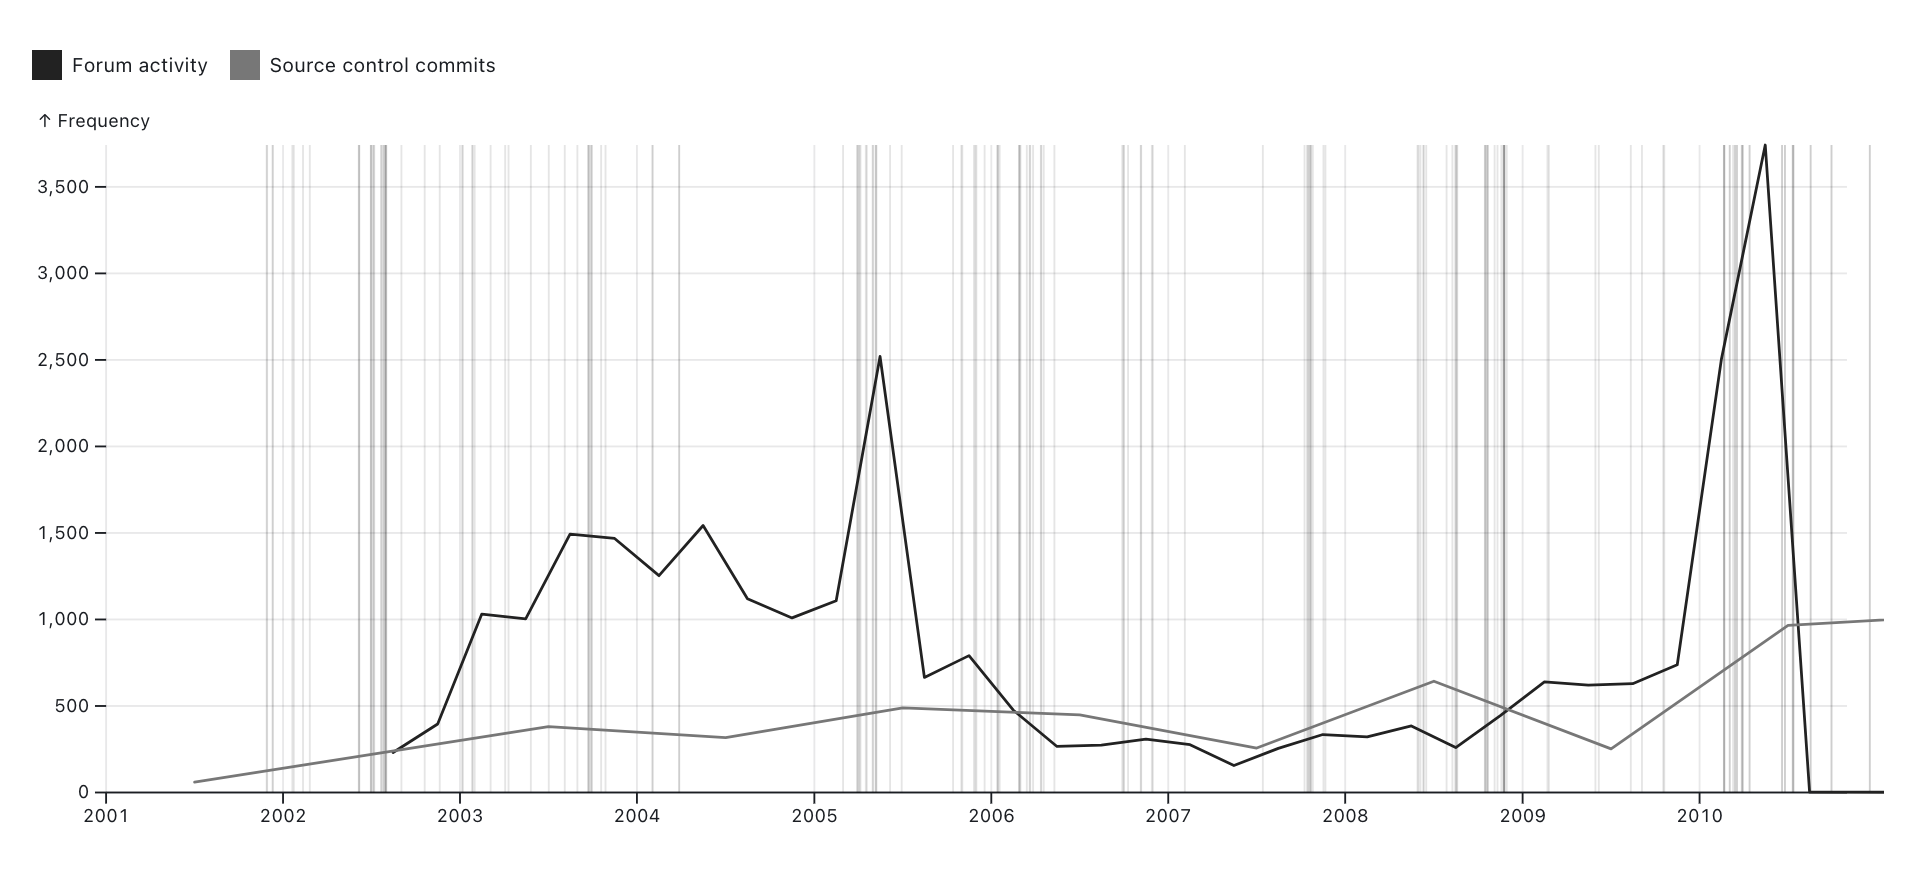
\includegraphics[width=1\textwidth]{images/figure-forum-git-activity.png} 

    \caption{Forum vs git activity vs releases (vertical lines)}
    \label{figure:forum-git-activity}  
  \end{figure}

There were 11,926 posts across 2,626 topics from 02/08/2002, 15:29 to the 19/04/2005, 09:55 across 1039 authors in the forum.

The alpha forum was a YaBB (Yet another Bulletin Board), it was seperated into forums which conained boards which contained topics which contained posts.

Similarly, Andreas Schlegel created the OSC P5 library as part of his final year project, reflecting a more academic-driven involvement. Schlegel's work on this library, stemming from his educational pursuits, highlights a focus on project-specific needs over community engagement in forums​​.

Complementing this, Simon Greenwold's contributions to Processing were significantly shaped by his academic and teaching roles. His time at the MIT Media Lab, interacting with the Aesthetics and Computation Group under John Maeda and corresponding with Processing's co-founders, Ben Fry and Casey Reas, provided a rich backdrop for his technical development. Greenwold worked on core aspects like the camera and lights in Processing and developed a particle system physics library, primarily for teaching purposes. His approach to the Processing community was less about forum participation and more focused on the technical and educational aspects, aligning with his background at institutions like Harvard and his lack of substantial engagement in online forums and communities​​​​.

In essence, Marxer, Schlegel, and Greenwold's deep-rooted academic and professional settings shaped their contributions to Processing differently than forum-centric members like Malka and Schwartz. These contributors were less reliant on the Processing forums for community support and interaction, focusing more on leveraging Processing in their academic and teaching activities. This delineation highlights the diverse motivations and environments influencing the engagements and contributions within the Processing community, ranging from community-driven interaction to academic and technical innovation.

